% Options for packages loaded elsewhere
\PassOptionsToPackage{unicode}{hyperref}
\PassOptionsToPackage{hyphens}{url}
%
\documentclass[
  english,
  man]{apa6}
\usepackage{lmodern}
\usepackage{amssymb,amsmath}
\usepackage{ifxetex,ifluatex}
\ifnum 0\ifxetex 1\fi\ifluatex 1\fi=0 % if pdftex
  \usepackage[T1]{fontenc}
  \usepackage[utf8]{inputenc}
  \usepackage{textcomp} % provide euro and other symbols
\else % if luatex or xetex
  \usepackage{unicode-math}
  \defaultfontfeatures{Scale=MatchLowercase}
  \defaultfontfeatures[\rmfamily]{Ligatures=TeX,Scale=1}
\fi
% Use upquote if available, for straight quotes in verbatim environments
\IfFileExists{upquote.sty}{\usepackage{upquote}}{}
\IfFileExists{microtype.sty}{% use microtype if available
  \usepackage[]{microtype}
  \UseMicrotypeSet[protrusion]{basicmath} % disable protrusion for tt fonts
}{}
\makeatletter
\@ifundefined{KOMAClassName}{% if non-KOMA class
  \IfFileExists{parskip.sty}{%
    \usepackage{parskip}
  }{% else
    \setlength{\parindent}{0pt}
    \setlength{\parskip}{6pt plus 2pt minus 1pt}}
}{% if KOMA class
  \KOMAoptions{parskip=half}}
\makeatother
\usepackage{xcolor}
\IfFileExists{xurl.sty}{\usepackage{xurl}}{} % add URL line breaks if available
\IfFileExists{bookmark.sty}{\usepackage{bookmark}}{\usepackage{hyperref}}
\hypersetup{
  pdftitle={The title},
  pdfauthor={Ouafaa Hmaddi1},
  pdfkeywords={keywords},
  hidelinks,
  pdfcreator={LaTeX via pandoc}}
\urlstyle{same} % disable monospaced font for URLs
\usepackage{graphicx,grffile}
\makeatletter
\def\maxwidth{\ifdim\Gin@nat@width>\linewidth\linewidth\else\Gin@nat@width\fi}
\def\maxheight{\ifdim\Gin@nat@height>\textheight\textheight\else\Gin@nat@height\fi}
\makeatother
% Scale images if necessary, so that they will not overflow the page
% margins by default, and it is still possible to overwrite the defaults
% using explicit options in \includegraphics[width, height, ...]{}
\setkeys{Gin}{width=\maxwidth,height=\maxheight,keepaspectratio}
% Set default figure placement to htbp
\makeatletter
\def\fps@figure{htbp}
\makeatother
\setlength{\emergencystretch}{3em} % prevent overfull lines
\providecommand{\tightlist}{%
  \setlength{\itemsep}{0pt}\setlength{\parskip}{0pt}}
\setcounter{secnumdepth}{-\maxdimen} % remove section numbering
% Make \paragraph and \subparagraph free-standing
\ifx\paragraph\undefined\else
  \let\oldparagraph\paragraph
  \renewcommand{\paragraph}[1]{\oldparagraph{#1}\mbox{}}
\fi
\ifx\subparagraph\undefined\else
  \let\oldsubparagraph\subparagraph
  \renewcommand{\subparagraph}[1]{\oldsubparagraph{#1}\mbox{}}
\fi
% Manuscript styling
\usepackage{upgreek}
\captionsetup{font=singlespacing,justification=justified}

% Table formatting
\usepackage{longtable}
\usepackage{lscape}
% \usepackage[counterclockwise]{rotating}   % Landscape page setup for large tables
\usepackage{multirow}		% Table styling
\usepackage{tabularx}		% Control Column width
\usepackage[flushleft]{threeparttable}	% Allows for three part tables with a specified notes section
\usepackage{threeparttablex}            % Lets threeparttable work with longtable

% Create new environments so endfloat can handle them
% \newenvironment{ltable}
%   {\begin{landscape}\begin{center}\begin{threeparttable}}
%   {\end{threeparttable}\end{center}\end{landscape}}
\newenvironment{lltable}{\begin{landscape}\begin{center}\begin{ThreePartTable}}{\end{ThreePartTable}\end{center}\end{landscape}}

% Enables adjusting longtable caption width to table width
% Solution found at http://golatex.de/longtable-mit-caption-so-breit-wie-die-tabelle-t15767.html
\makeatletter
\newcommand\LastLTentrywidth{1em}
\newlength\longtablewidth
\setlength{\longtablewidth}{1in}
\newcommand{\getlongtablewidth}{\begingroup \ifcsname LT@\roman{LT@tables}\endcsname \global\longtablewidth=0pt \renewcommand{\LT@entry}[2]{\global\advance\longtablewidth by ##2\relax\gdef\LastLTentrywidth{##2}}\@nameuse{LT@\roman{LT@tables}} \fi \endgroup}

% \setlength{\parindent}{0.5in}
% \setlength{\parskip}{0pt plus 0pt minus 0pt}

% \usepackage{etoolbox}
\makeatletter
\patchcmd{\HyOrg@maketitle}
  {\section{\normalfont\normalsize\abstractname}}
  {\section*{\normalfont\normalsize\abstractname}}
  {}{\typeout{Failed to patch abstract.}}
\patchcmd{\HyOrg@maketitle}
  {\section{\protect\normalfont{\@title}}}
  {\section*{\protect\normalfont{\@title}}}
  {}{\typeout{Failed to patch title.}}
\makeatother
\shorttitle{Title}
\keywords{keywords\newline\indent Word count: X}
\DeclareDelayedFloatFlavor{ThreePartTable}{table}
\DeclareDelayedFloatFlavor{lltable}{table}
\DeclareDelayedFloatFlavor*{longtable}{table}
\makeatletter
\renewcommand{\efloat@iwrite}[1]{\immediate\expandafter\protected@write\csname efloat@post#1\endcsname{}}
\makeatother
\usepackage{lineno}

\linenumbers
\usepackage{csquotes}
\ifxetex
  % Load polyglossia as late as possible: uses bidi with RTL langages (e.g. Hebrew, Arabic)
  \usepackage{polyglossia}
  \setmainlanguage[]{english}
\else
  \usepackage[shorthands=off,main=english]{babel}
\fi

\title{The title}
\author{Ouafaa Hmaddi\textsuperscript{1}}
\date{}


\authornote{

Add complete departmental affiliations for each author here. Each new line herein must be indented, like this line.

Enter author note here.

The authors made the following contributions. Ouafaa Hmaddi: Conceptualization, Writing - Original Draft Preparation, Writing - Review \& Editing.

Correspondence concerning this article should be addressed to Ouafaa Hmaddi, Postal address. E-mail: \href{mailto:ohmaddi@uoregon.edu}{\nolinkurl{ohmaddi@uoregon.edu}}

}

\affiliation{\vspace{0.5cm}\textsuperscript{1} University of Oregon}

\abstract{
One or two sentences providing a \textbf{basic introduction} to the field, comprehensible to a scientist in any discipline.

Two to three sentences of \textbf{more detailed background}, comprehensible to scientists in related disciplines.

One sentence clearly stating the \textbf{general problem} being addressed by this particular study.

One sentence summarizing the main result (with the words ``\textbf{here we show}'' or their equivalent).

Two or three sentences explaining what the \textbf{main result} reveals in direct comparison to what was thought to be the case previously, or how the main result adds to previous knowledge.

One or two sentences to put the results into a more \textbf{general context}.

Two or three sentences to provide a \textbf{broader perspective}, readily comprehensible to a scientist in any discipline.
}



\begin{document}
\maketitle

\hypertarget{methods}{%
\section{Methods}\label{methods}}

We report how we determined our sample size, all data exclusions (if any), all manipulations, and all measures in the study.

\hypertarget{participants}{%
\subsection{Participants}\label{participants}}

\hypertarget{material}{%
\subsection{Material}\label{material}}

\hypertarget{procedure}{%
\subsection{Procedure}\label{procedure}}

\hypertarget{data-analysis}{%
\subsection{Data analysis}\label{data-analysis}}

We used R (Version 4.0.2; R Core Team, 2020) and the R-packages \emph{lme4} (Version 1.1.23; Bates, Mächler, Bolker, \& Walker, 2015), \emph{Matrix} (Version 1.2.18; Bates \& Maechler, 2019), and \emph{papaja} (Version 0.1.0.9997; Aust \& Barth, 2020) for all our analyses.

\#CGI data

\#Plotting all countries along the 3 dimensions

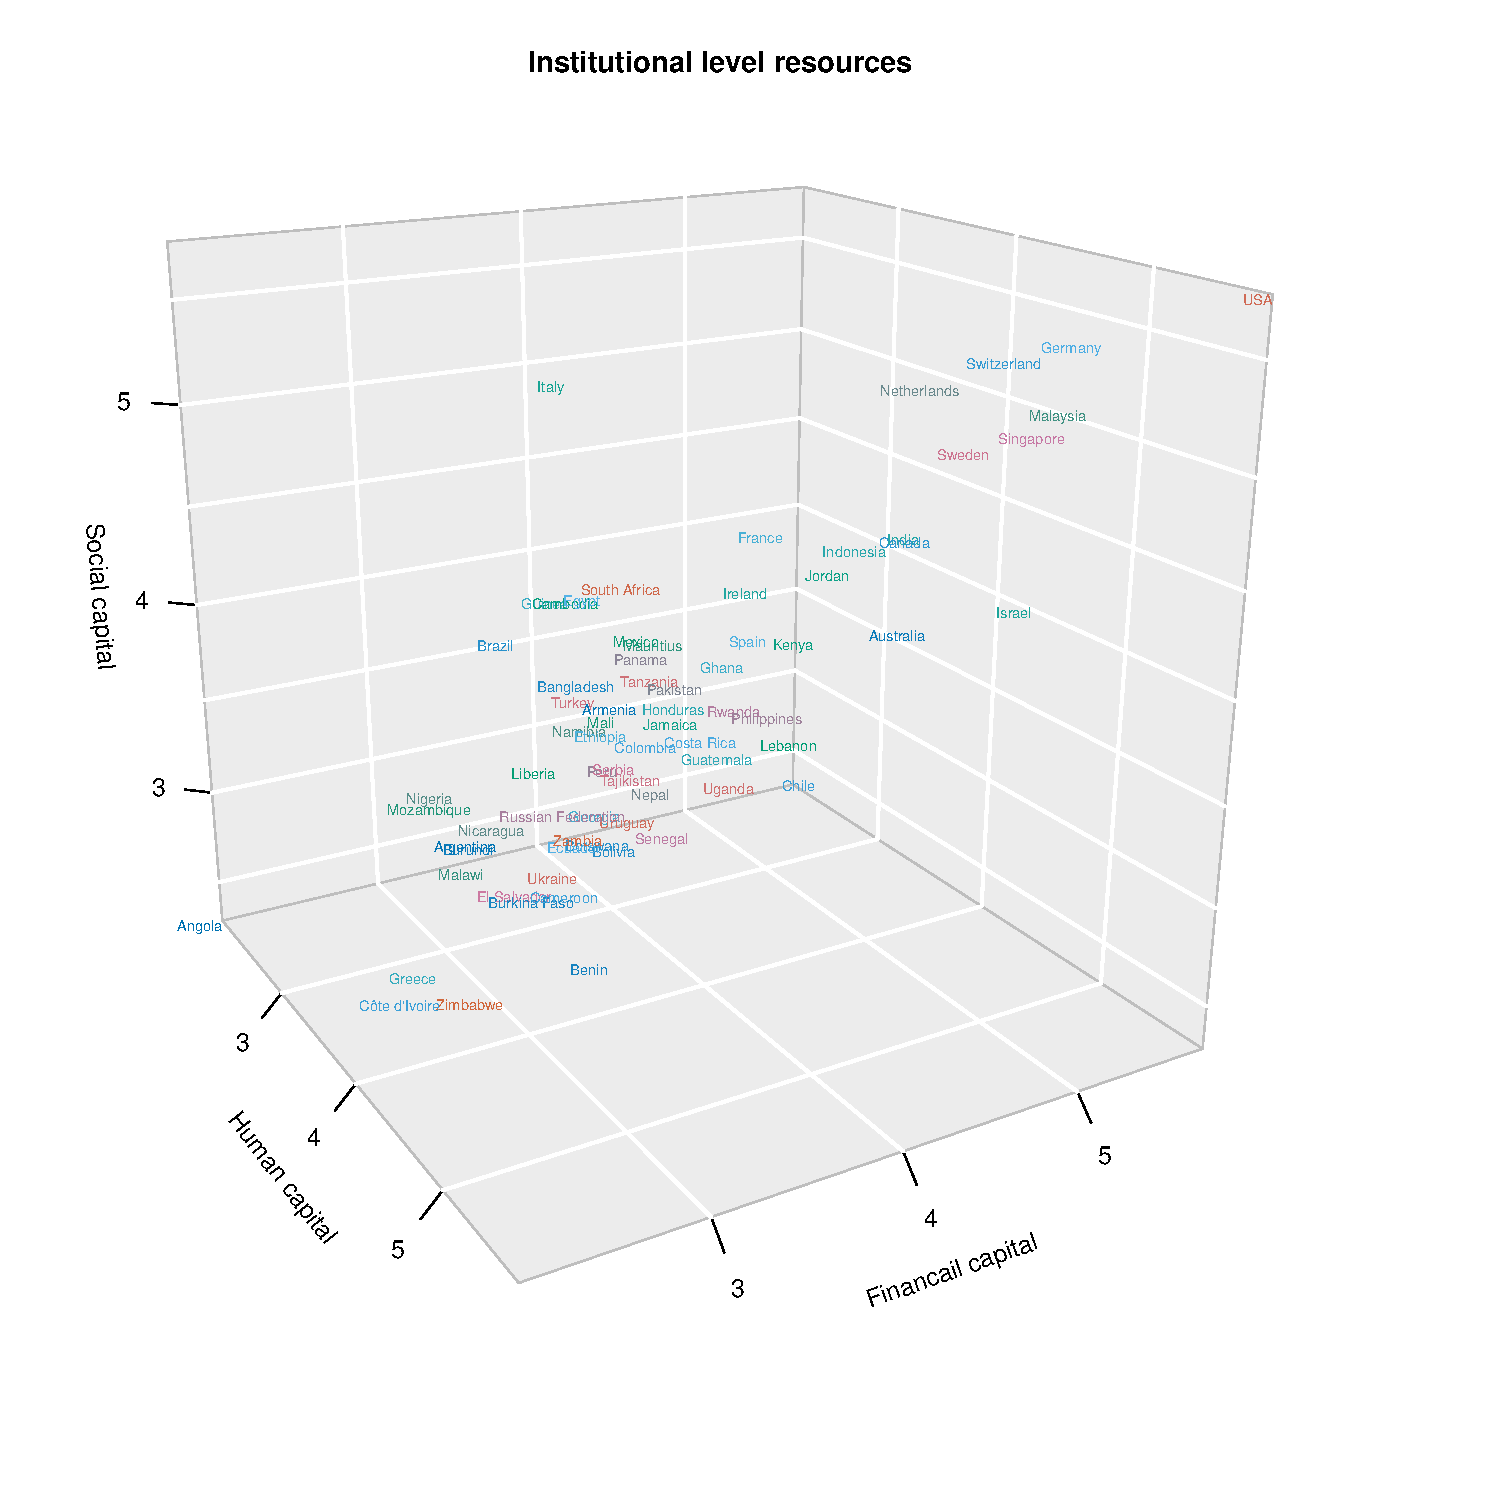
\includegraphics{Manuscript_files/figure-latex/unnamed-chunk-4-1.pdf} 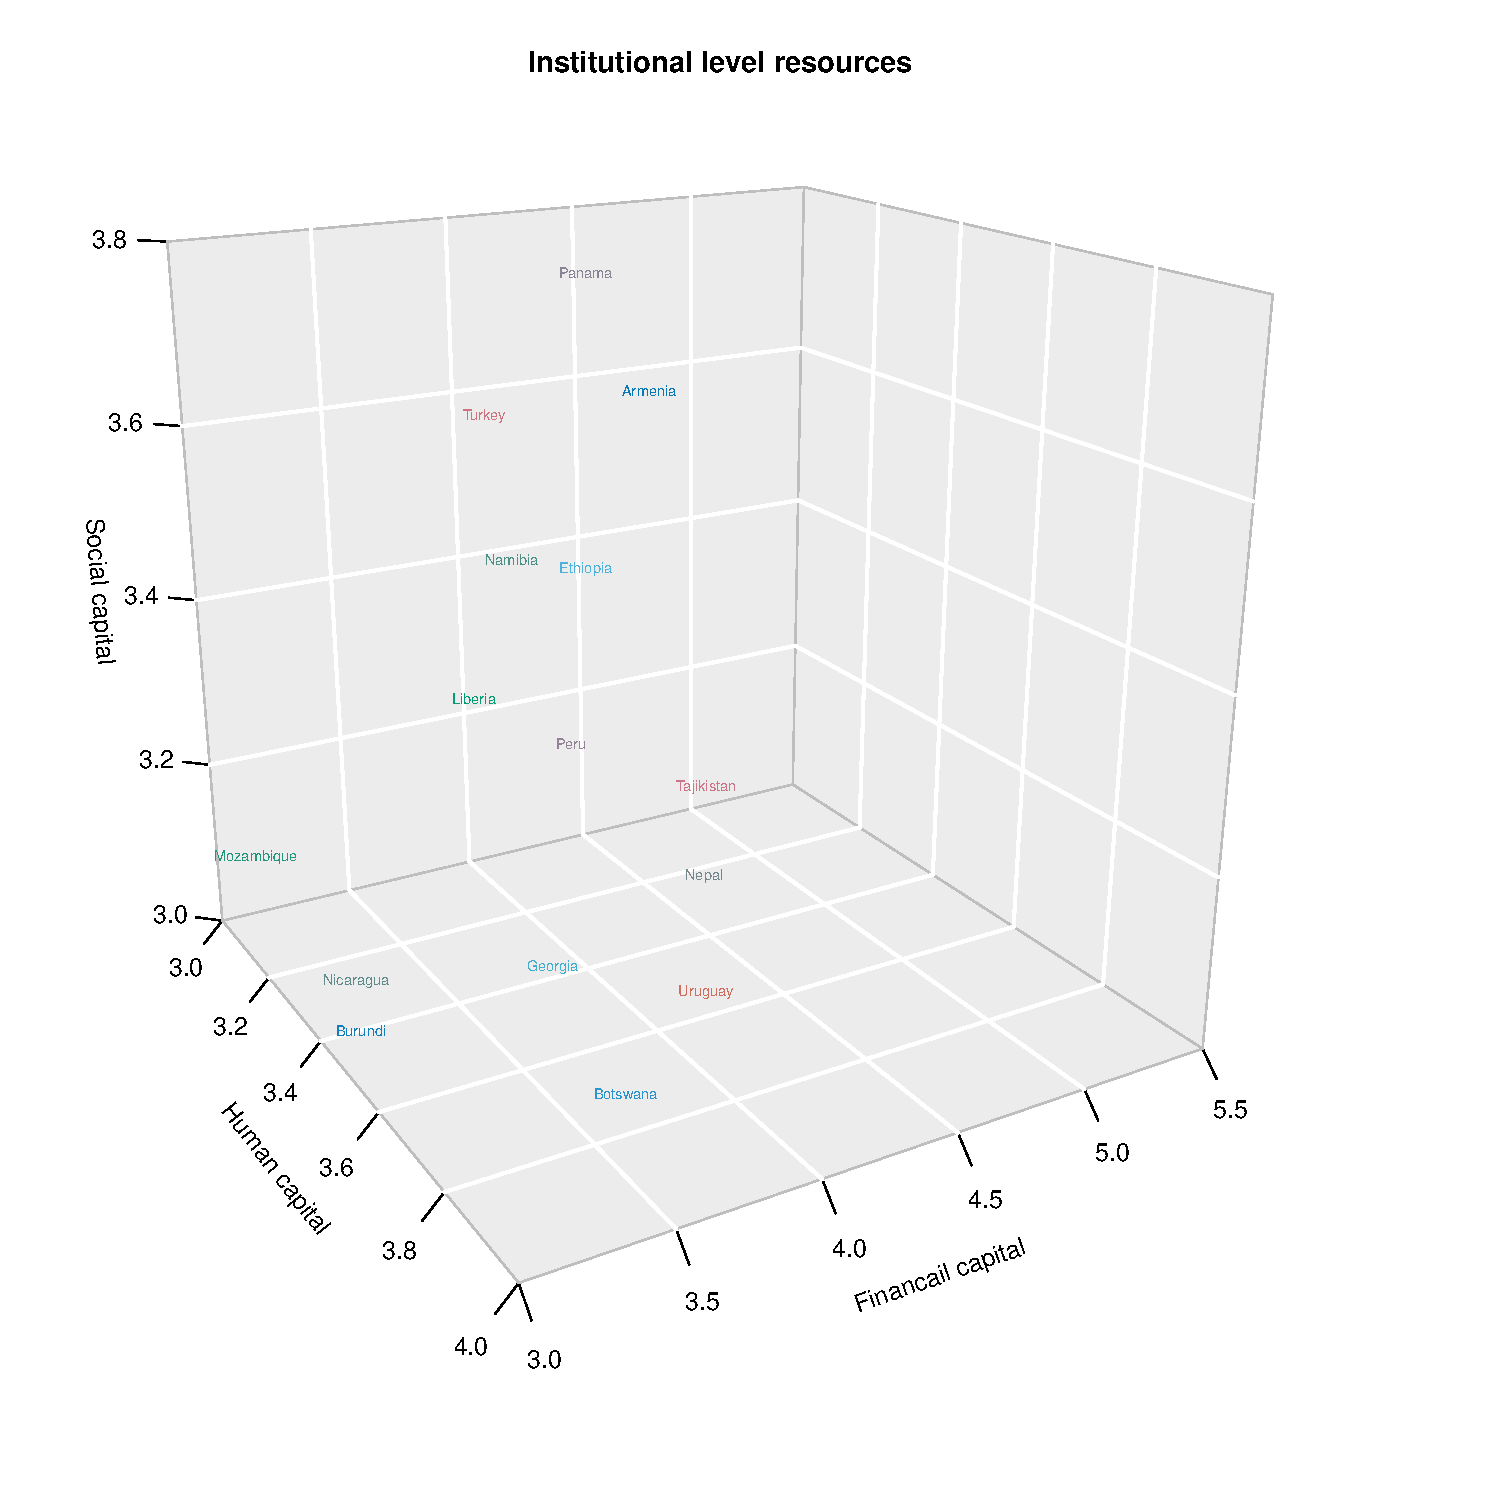
\includegraphics{Manuscript_files/figure-latex/unnamed-chunk-4-2.pdf}

\#Attention to capital - venture data

\#Reverse code attention variable

\#Join all 3 datasets

\#Fiancial Capital acquisiton total

\#Revenues

\#Human capital acquisition

\#Social capital acquisition

\hypertarget{results}{%
\section{Results}\label{results}}

\#Mixed model analysis - Human capital

\begin{tabular}{l|l|l|l}
\hline
  & \$b\$ & SE & \$z\$\\
\hline
Intercept & -1.47 & 0.08 & -19.16\\
\hline
Attention to Human capital(AHC) & 0.10 & 0.08 & 1.24\\
\hline
\end{tabular}

\begin{tabular}{l|l|l|l}
\hline
  & \$b\$ & SE & \$z\$\\
\hline
Intercept & -0.94 & 0.53 & -1.77\\
\hline
AHC & 0.86 & 0.44 & 1.97\\
\hline
Ease of finding skilled employees & -0.12 & 0.12 & -0.96\\
\hline
AHCxEase of finding skilled employees & -0.16 & 0.09 & -1.69\\
\hline
\end{tabular}

\begin{tabular}{l|l|l|l}
\hline
  & \$b\$ & SE & \$t\$\\
\hline
Intercept & 738.20 & 485.65 & 1.52\\
\hline
Attention to Human capital & 2,841.44 & 2,153.75 & 1.32\\
\hline
\end{tabular}

\begin{tabular}{l|l|l|l}
\hline
  & \$b\$ & SE & \$t\$\\
\hline
Intercept & -1,882.79 & 3,470.12 & -0.54\\
\hline
AHC & -9,744.87 & 16,027.75 & -0.61\\
\hline
Ease of finding skilled employees & 618.05 & 783.89 & 0.79\\
\hline
AHCxEase of finding skilled employees & 2,989.85 & 3,687.09 & 0.81\\
\hline
\end{tabular}

\#Mixed model analysis - Financial capital

\begin{verbatim}
## Linear mixed model fit by maximum likelihood  ['lmerMod']
## Formula: participated ~ +(accel_ben_rank_direct_funding | country)
##    Data: gali_joined
## 
##      AIC      BIC   logLik deviance df.resid 
##  14831.2  14869.8  -7410.6  14821.2    16439 
## 
## Scaled residuals: 
##     Min      1Q  Median      3Q     Max 
## -1.3463 -0.5096 -0.4046 -0.2890  2.4564 
## 
## Random effects:
##  Groups   Name                          Variance Std.Dev. Corr 
##  country  (Intercept)                   0.008936 0.09453       
##           accel_ben_rank_direct_funding 0.001665 0.04080  -0.49
##  Residual                               0.142950 0.37809       
## Number of obs: 16444, groups:  country, 83
## 
## Fixed effects:
##             Estimate Std. Error t value
## (Intercept)  0.19651    0.01228   16.01
\end{verbatim}

\begin{verbatim}
## Linear mixed model fit by maximum likelihood  ['lmerMod']
## Formula: 
## participated ~ accel_ben_rank_direct_funding * EOSQ425 + (accel_ben_rank_direct_funding |  
##     country)
##    Data: gali_joined
## 
##      AIC      BIC   logLik deviance df.resid 
##  14620.0  14681.5  -7302.0  14604.0    16177 
## 
## Scaled residuals: 
##     Min      1Q  Median      3Q     Max 
## -1.4017 -0.5138 -0.3955 -0.2813  2.4249 
## 
## Random effects:
##  Groups   Name                          Variance  Std.Dev. Corr 
##  country  (Intercept)                   0.0085583 0.09251       
##           accel_ben_rank_direct_funding 0.0009436 0.03072  -1.00
##  Residual                               0.1432556 0.37849       
## Number of obs: 16185, groups:  country, 74
## 
## Fixed effects:
##                                         Estimate Std. Error t value
## (Intercept)                            0.2004428  0.0710787   2.820
## accel_ben_rank_direct_funding         -0.0255510  0.0455072  -0.561
## EOSQ425                                0.0008104  0.0184340   0.044
## accel_ben_rank_direct_funding:EOSQ425 -0.0023544  0.0107909  -0.218
## 
## Correlation of Fixed Effects:
##             (Intr) ac____ EOSQ42
## accl_bn_r__ -0.490              
## EOSQ425     -0.984  0.485       
## a____:EOSQ4  0.533 -0.975 -0.545
## convergence code: 0
## boundary (singular) fit: see ?isSingular
\end{verbatim}

\begin{verbatim}
## Linear mixed model fit by maximum likelihood  ['lmerMod']
## Formula: 
## participated ~ accel_ben_rank_direct_funding * EOSQ089 + (accel_ben_rank_direct_funding |  
##     country)
##    Data: gali_joined
## 
##      AIC      BIC   logLik deviance df.resid 
##  14619.7  14681.2  -7301.8  14603.7    16177 
## 
## Scaled residuals: 
##     Min      1Q  Median      3Q     Max 
## -1.4020 -0.5136 -0.3962 -0.2810  2.4270 
## 
## Random effects:
##  Groups   Name                          Variance  Std.Dev. Corr 
##  country  (Intercept)                   0.0084870 0.09212       
##           accel_ben_rank_direct_funding 0.0009291 0.03048  -1.00
##  Residual                               0.1432565 0.37849       
## Number of obs: 16185, groups:  country, 74
## 
## Fixed effects:
##                                        Estimate Std. Error t value
## (Intercept)                            0.229561   0.046331   4.955
## accel_ben_rank_direct_funding         -0.037525   0.030596  -1.226
## EOSQ089                               -0.008695   0.014873  -0.585
## accel_ben_rank_direct_funding:EOSQ089  0.001088   0.008465   0.129
## 
## Correlation of Fixed Effects:
##             (Intr) ac____ EOSQ08
## accl_bn_r__ -0.477              
## EOSQ089     -0.961  0.464       
## a____:EOSQ0  0.539 -0.944 -0.566
## convergence code: 0
## boundary (singular) fit: see ?isSingular
\end{verbatim}

\begin{verbatim}
## Linear mixed model fit by maximum likelihood  ['lmerMod']
## Formula: participated ~ accel_ben_rank_direct_funding * DOMCREDITGDP +  
##     (accel_ben_rank_direct_funding | country)
##    Data: gali_joined
## 
##      AIC      BIC   logLik deviance df.resid 
##  14619.7  14681.2  -7301.8  14603.7    16177 
## 
## Scaled residuals: 
##     Min      1Q  Median      3Q     Max 
## -1.3992 -0.5115 -0.3980 -0.2807  2.4272 
## 
## Random effects:
##  Groups   Name                          Variance  Std.Dev. Corr 
##  country  (Intercept)                   0.0085682 0.09256       
##           accel_ben_rank_direct_funding 0.0009053 0.03009  -1.00
##  Residual                               0.1432523 0.37849       
## Number of obs: 16185, groups:  country, 74
## 
## Fixed effects:
##                                              Estimate Std. Error t value
## (Intercept)                                 2.113e-01  2.084e-02  10.137
## accel_ben_rank_direct_funding              -3.313e-02  1.549e-02  -2.139
## DOMCREDITGDP                               -1.339e-04  2.829e-04  -0.473
## accel_ben_rank_direct_funding:DOMCREDITGDP -1.288e-05  1.590e-04  -0.081
## 
## Correlation of Fixed Effects:
##             (Intr) ac____ DOMCRE
## accl_bn_r__ -0.414              
## DOMCREDITGD -0.788  0.334       
## a____:DOMCR  0.441 -0.768 -0.567
## convergence code: 0
## boundary (singular) fit: see ?isSingular
\end{verbatim}

\begin{verbatim}
## Linear mixed model fit by maximum likelihood  ['lmerMod']
## Formula: capital_raised_tot ~ +(accel_ben_rank_direct_funding | country)
##    Data: gali_joined
## 
##       AIC       BIC    logLik  deviance  df.resid 
##  628881.3  628919.9 -314435.7  628871.3     16439 
## 
## Scaled residuals: 
##     Min      1Q  Median      3Q     Max 
##  -0.756  -0.010  -0.008  -0.004 126.757 
## 
## Random effects:
##  Groups   Name                          Variance  Std.Dev. Corr 
##  country  (Intercept)                   1.168e+13  3417674      
##           accel_ben_rank_direct_funding 4.366e+13  6607224 -1.00
##  Residual                               2.373e+15 48709324      
## Number of obs: 16444, groups:  country, 83
## 
## Fixed effects:
##             Estimate Std. Error t value
## (Intercept)   607877     562167   1.081
## convergence code: 0
## boundary (singular) fit: see ?isSingular
\end{verbatim}

\begin{verbatim}
## Linear mixed model fit by maximum likelihood  ['lmerMod']
## Formula: capital_raised_tot ~ accel_ben_rank_direct_funding * EOSQ425 +  
##     (accel_ben_rank_direct_funding | country)
##    Data: gali_joined
## 
##       AIC       BIC    logLik  deviance  df.resid 
##  619237.1  619298.6 -309610.6  619221.1     16177 
## 
## Scaled residuals: 
##     Min      1Q  Median      3Q     Max 
##  -0.770  -0.009  -0.006  -0.004 125.749 
## 
## Random effects:
##  Groups   Name                          Variance  Std.Dev. Corr 
##  country  (Intercept)                   1.205e+13  3471900      
##           accel_ben_rank_direct_funding 4.540e+13  6737688 -1.00
##  Residual                               2.410e+15 49094901      
## Number of obs: 16185, groups:  country, 74
## 
## Fixed effects:
##                                       Estimate Std. Error t value
## (Intercept)                            3278060    3931054   0.834
## accel_ben_rank_direct_funding         -5097275    8516455  -0.599
## EOSQ425                                -589495    1003353  -0.588
## accel_ben_rank_direct_funding:EOSQ425   972897    2131244   0.456
## 
## Correlation of Fixed Effects:
##             (Intr) ac____ EOSQ42
## accl_bn_r__ -0.717              
## EOSQ425     -0.982  0.725       
## a____:EOSQ4  0.740 -0.980 -0.771
## convergence code: 0
## boundary (singular) fit: see ?isSingular
\end{verbatim}

\begin{verbatim}
## Linear mixed model fit by maximum likelihood  ['lmerMod']
## Formula: capital_raised_tot ~ accel_ben_rank_direct_funding * EOSQ089 +  
##     (accel_ben_rank_direct_funding | country)
##    Data: gali_joined
## 
##       AIC       BIC    logLik  deviance  df.resid 
##  619236.9  619298.5 -309610.5  619220.9     16177 
## 
## Scaled residuals: 
##     Min      1Q  Median      3Q     Max 
##  -0.771  -0.009  -0.006  -0.004 125.749 
## 
## Random effects:
##  Groups   Name                          Variance  Std.Dev. Corr 
##  country  (Intercept)                   1.196e+13  3458659      
##           accel_ben_rank_direct_funding 4.502e+13  6709707 -1.00
##  Residual                               2.410e+15 49094926      
## Number of obs: 16185, groups:  country, 74
## 
## Fixed effects:
##                                       Estimate Std. Error t value
## (Intercept)                            2758748    2542379   1.085
## accel_ben_rank_direct_funding         -4463383    5575404  -0.801
## EOSQ089                                -575121     797830  -0.721
## accel_ben_rank_direct_funding:EOSQ089  1016469    1690294   0.601
## 
## Correlation of Fixed Effects:
##             (Intr) ac____ EOSQ08
## accl_bn_r__ -0.700              
## EOSQ089     -0.957  0.703       
## a____:EOSQ0  0.729 -0.952 -0.787
## convergence code: 0
## boundary (singular) fit: see ?isSingular
\end{verbatim}

\begin{verbatim}
## Linear mixed model fit by maximum likelihood  ['lmerMod']
## Formula: capital_raised_tot ~ accel_ben_rank_direct_funding * DOMCREDITGDP +  
##     (accel_ben_rank_direct_funding | country)
##    Data: gali_joined
## 
##       AIC       BIC    logLik  deviance  df.resid 
##  619237.2  619298.7 -309610.6  619221.2     16177 
## 
## Scaled residuals: 
##     Min      1Q  Median      3Q     Max 
##  -0.770  -0.007  -0.006  -0.004 125.749 
## 
## Random effects:
##  Groups   Name                          Variance  Std.Dev. Corr 
##  country  (Intercept)                   1.208e+13  3475044      
##           accel_ben_rank_direct_funding 4.521e+13  6724103 -1.00
##  Residual                               2.410e+15 49095018      
## Number of obs: 16185, groups:  country, 74
## 
## Fixed effects:
##                                            Estimate Std. Error t value
## (Intercept)                                 1451825    1141899   1.271
## accel_ben_rank_direct_funding              -2232392    2605340  -0.857
## DOMCREDITGDP                                  -7480      14628  -0.511
## accel_ben_rank_direct_funding:DOMCREDITGDP    13756      31129   0.442
## 
## Correlation of Fixed Effects:
##             (Intr) ac____ DOMCRE
## accl_bn_r__ -0.615              
## DOMCREDITGD -0.764  0.519       
## a____:DOMCR  0.555 -0.760 -0.779
## convergence code: 0
## boundary (singular) fit: see ?isSingular
\end{verbatim}

\#Mixed model analysis - Social capital

\begin{verbatim}
##                          Estimate Std. Error   t value
## (Intercept)            0.20204321 0.01250494 16.157077
## accel_ben_rank_network 0.01914256 0.00950974  2.012943
\end{verbatim}

\begin{verbatim}
##                                    Estimate Std. Error    t value
## (Intercept)                     0.295903338 0.06852242  4.3183434
## accel_ben_rank_network          0.023874383 0.05035733  0.4740994
## EOSQ109                        -0.023521692 0.01733603 -1.3568099
## accel_ben_rank_network:EOSQ109 -0.001363126 0.01125294 -0.1211352
\end{verbatim}

\begin{verbatim}
##                          Estimate Std. Error   t value
## (Intercept)            0.57431349 0.04229280 13.579463
## accel_ben_rank_network 0.06431639 0.04574601  1.405945
\end{verbatim}

\begin{verbatim}
##                                  Estimate Std. Error   t value
## (Intercept)                    -0.2693634 0.20697678 -1.301419
## accel_ben_rank_network         -0.5635796 0.23434531 -2.404911
## EOSQ109                         0.2155408 0.05213442  4.134328
## accel_ben_rank_network:EOSQ109  0.1600702 0.05499693  2.910531
\end{verbatim}

\hypertarget{discussion}{%
\section{Discussion}\label{discussion}}

\newpage

\hypertarget{references}{%
\section{References}\label{references}}

\begingroup
\setlength{\parindent}{-0.5in}
\setlength{\leftskip}{0.5in}

\hypertarget{refs}{}
\leavevmode\hypertarget{ref-R-papaja}{}%
Aust, F., \& Barth, M. (2020). \emph{papaja: Create APA manuscripts with R Markdown}. Retrieved from \url{https://github.com/crsh/papaja}

\leavevmode\hypertarget{ref-R-Matrix}{}%
Bates, D., \& Maechler, M. (2019). \emph{Matrix: Sparse and dense matrix classes and methods}. Retrieved from \url{https://CRAN.R-project.org/package=Matrix}

\leavevmode\hypertarget{ref-R-lme4}{}%
Bates, D., Mächler, M., Bolker, B., \& Walker, S. (2015). Fitting linear mixed-effects models using lme4. \emph{Journal of Statistical Software}, \emph{67}(1), 1--48. \url{https://doi.org/10.18637/jss.v067.i01}

\leavevmode\hypertarget{ref-R-base}{}%
R Core Team. (2020). \emph{R: A language and environment for statistical computing}. Vienna, Austria: R Foundation for Statistical Computing. Retrieved from \url{https://www.R-project.org/}

\endgroup


\end{document}
